\begin{figure*}[!ht]
\centering
\setlength{\tabcolsep}{1pt}
\renewcommand{\arraystretch}{0.6}
\begin{tabular}{c@{\hspace{1pt}}cccc}
\rotatebox{90}{\,\textbf{NFIP Claims}} &
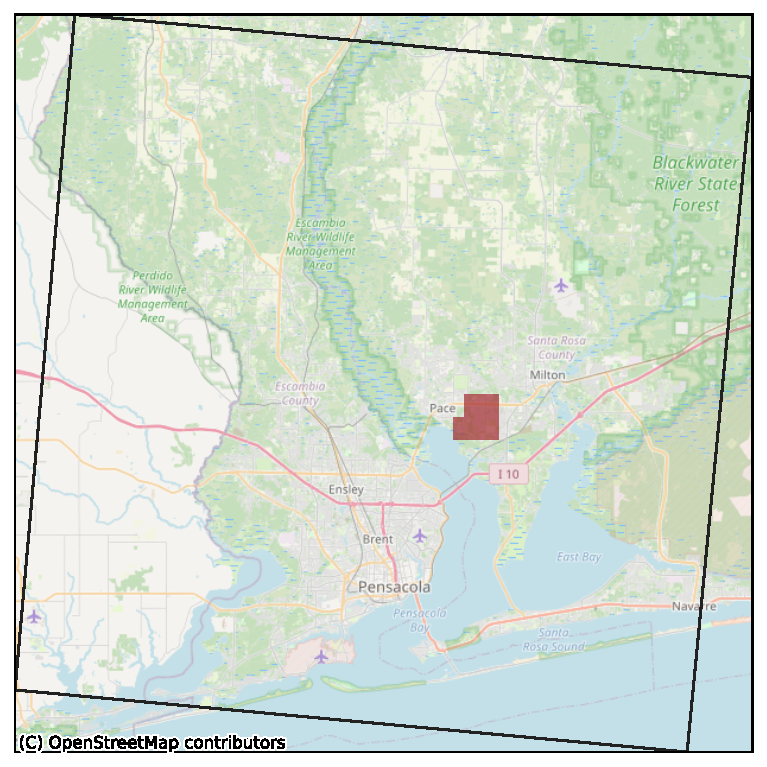
\includegraphics[width=0.22\textwidth]{figs/1_ob.pdf} &
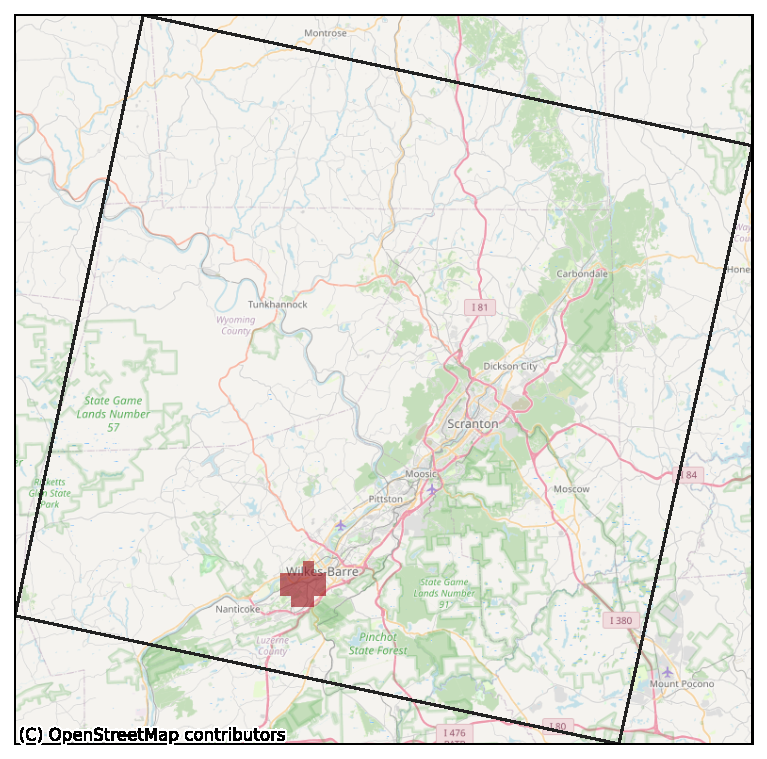
\includegraphics[width=0.22\textwidth]{figs/2_ob.pdf} &
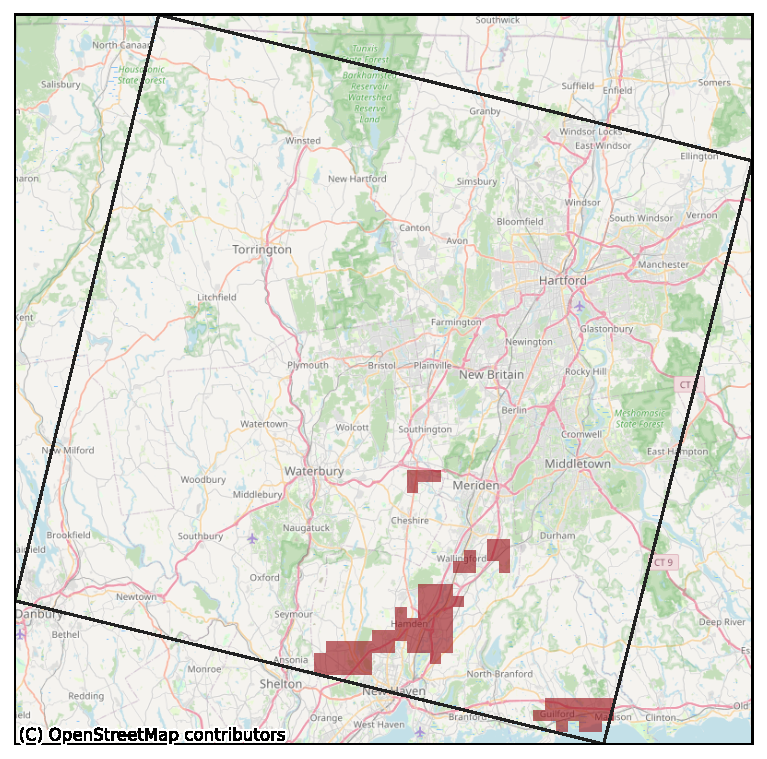
\includegraphics[width=0.22\textwidth]{figs/4_ob.pdf} &
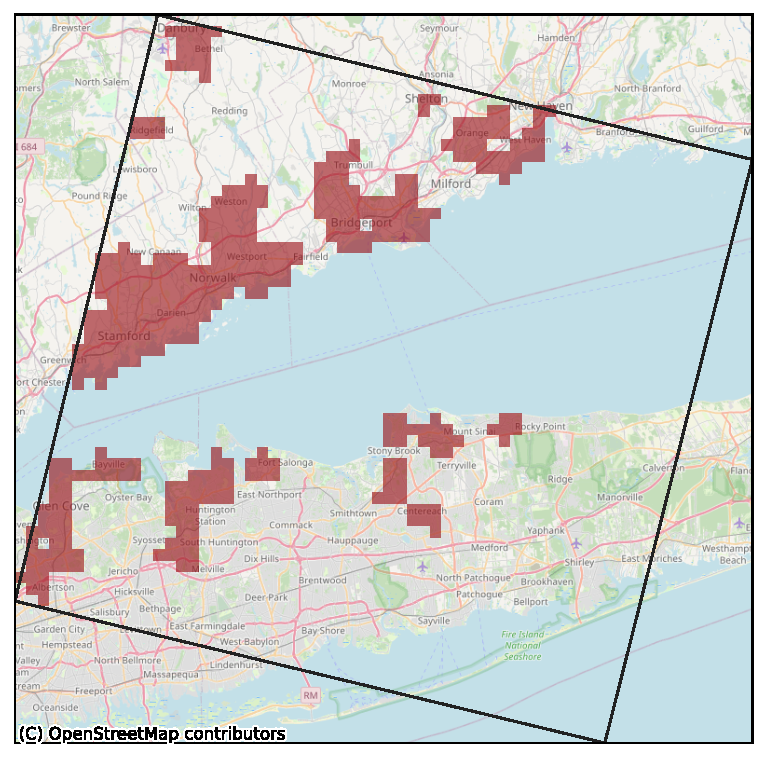
\includegraphics[width=0.22\textwidth]{figs/5_ob.pdf} \\
\rotatebox{90}{\,\textbf{Predicted}} &
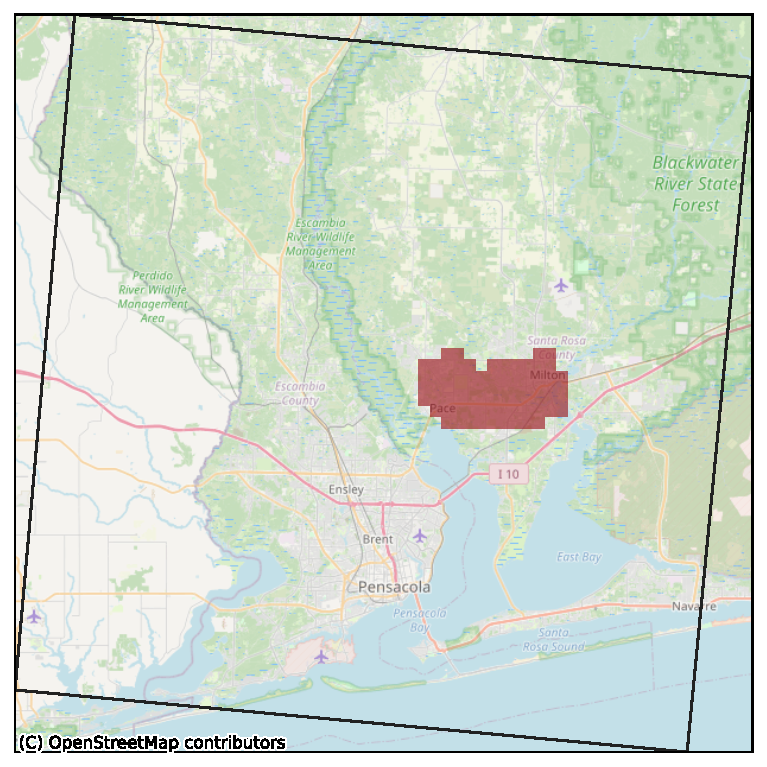
\includegraphics[width=0.22\textwidth]{figs/1_pred.pdf} &
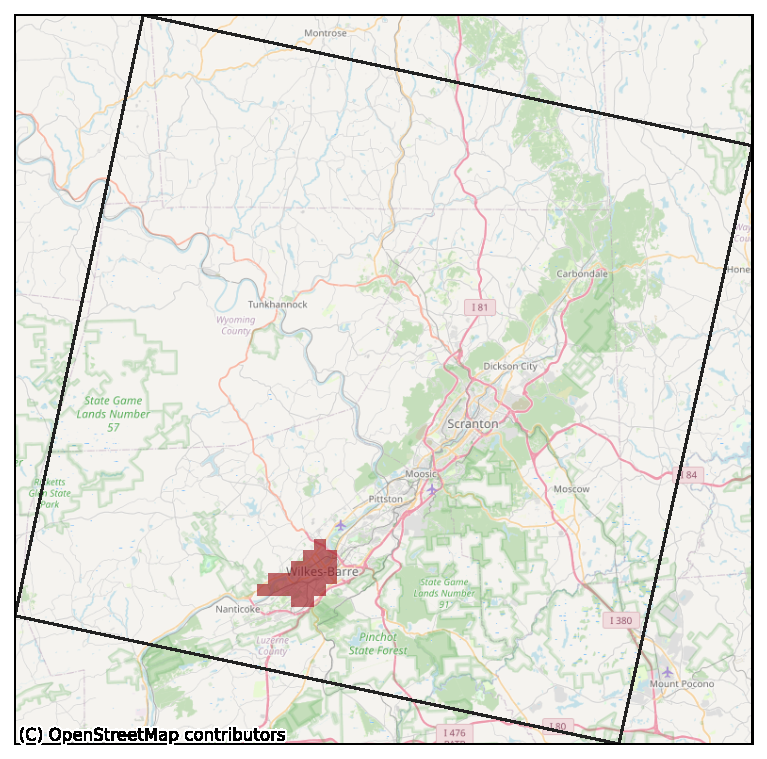
\includegraphics[width=0.22\textwidth]{figs/2_pred.pdf} &
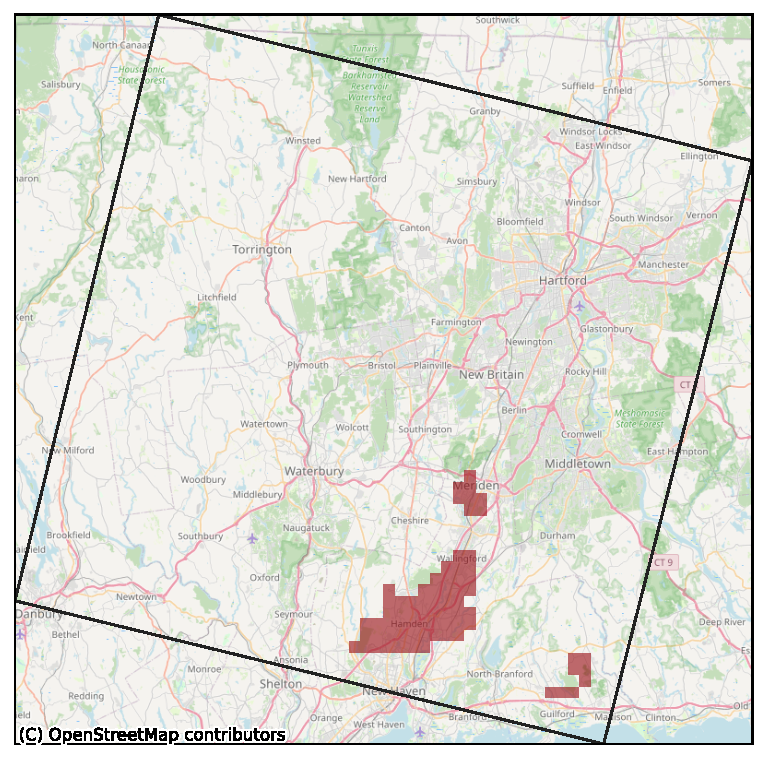
\includegraphics[width=0.22\textwidth]{figs/4_pred.pdf} &
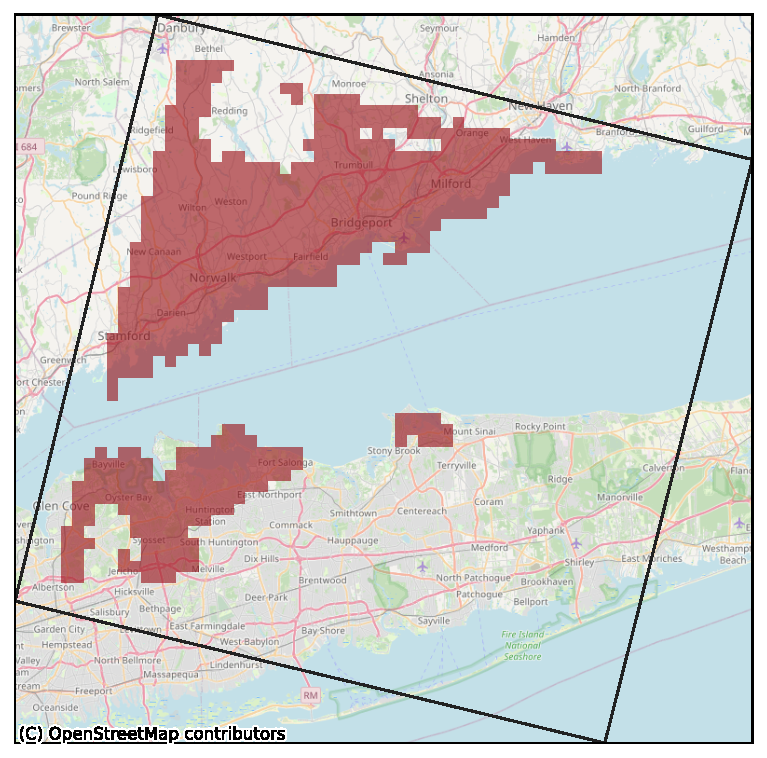
\includegraphics[width=0.22\textwidth]{figs/5_pred.pdf} \\
\end{tabular}

\vspace{4pt}

\begin{tabular}{c@{\hspace{1pt}}ccc}
\rotatebox{90}{\,\textbf{NFIP Claims}} &
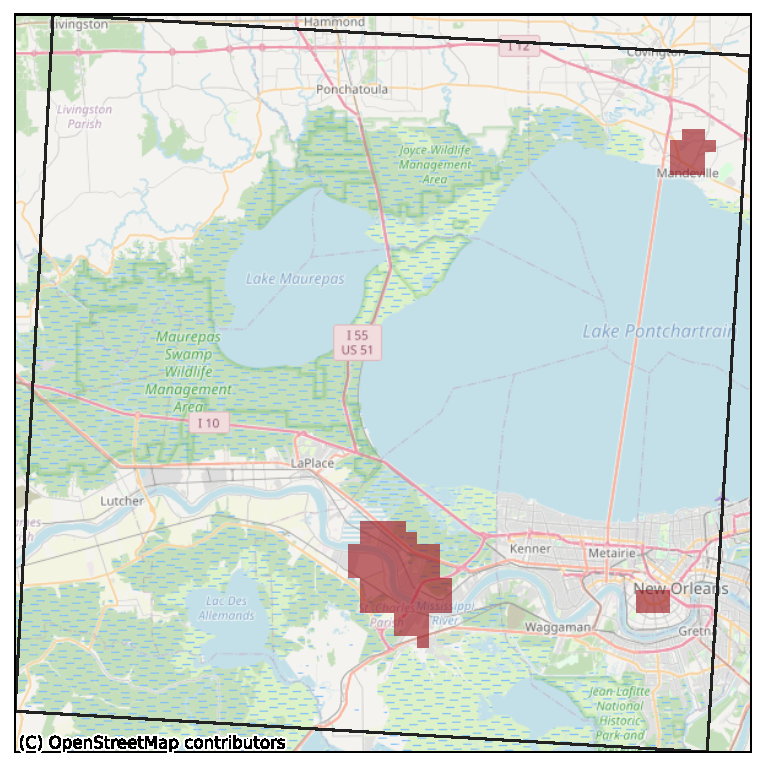
\includegraphics[width=0.22\textwidth]{figs/6_ob.pdf} &
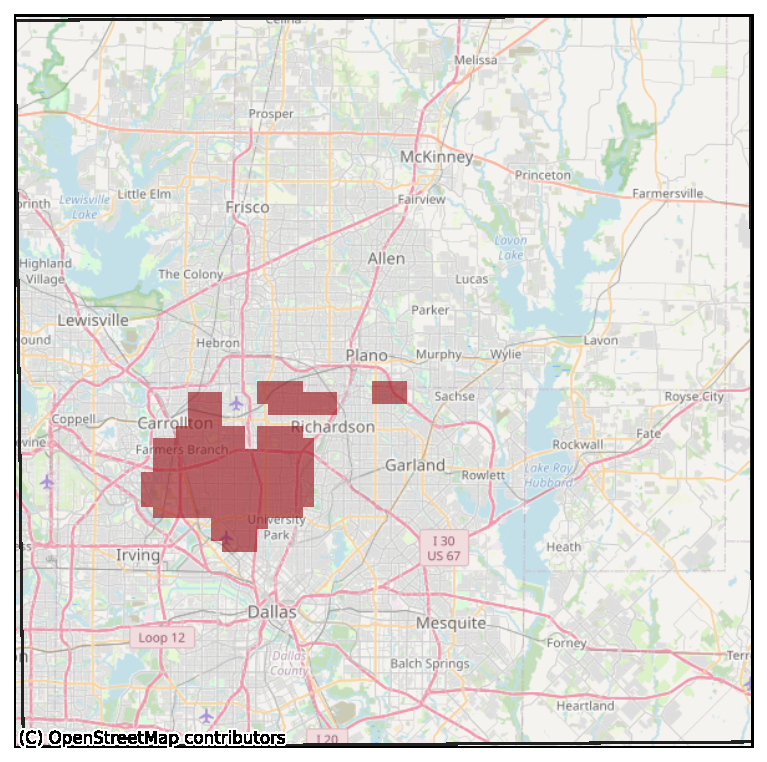
\includegraphics[width=0.22\textwidth]{figs/7_ob.pdf} &
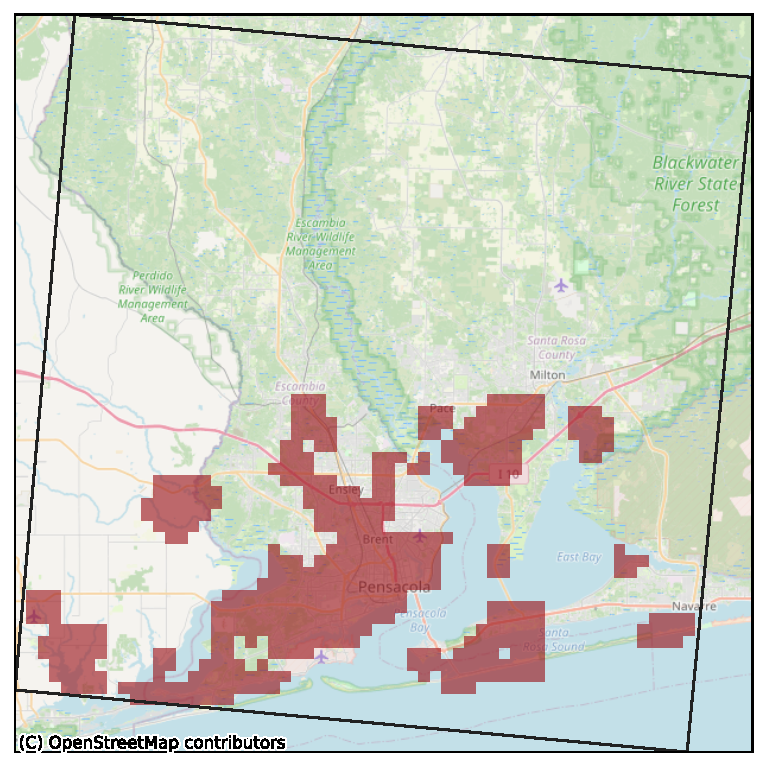
\includegraphics[width=0.22\textwidth]{figs/8_ob.pdf} \\
\rotatebox{90}{\,\textbf{Predicted}} &
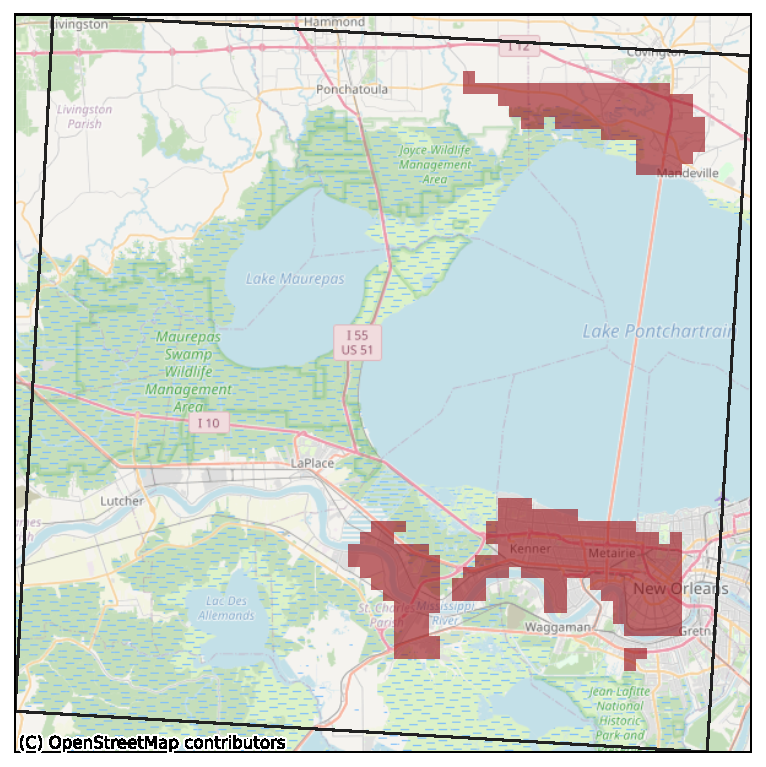
\includegraphics[width=0.22\textwidth]{figs/6_pred.pdf} &
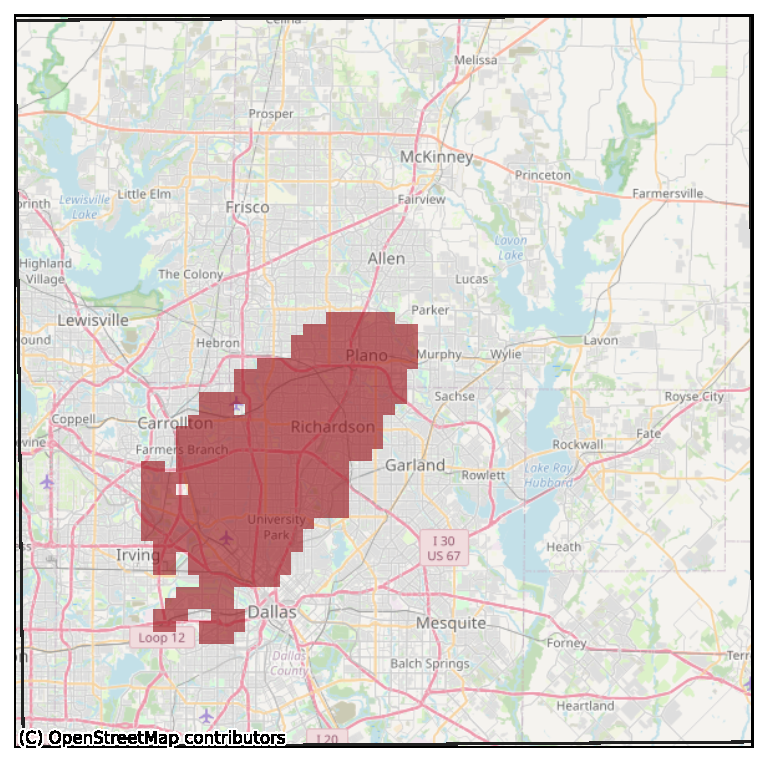
\includegraphics[width=0.22\textwidth]{figs/7_pred.pdf} &
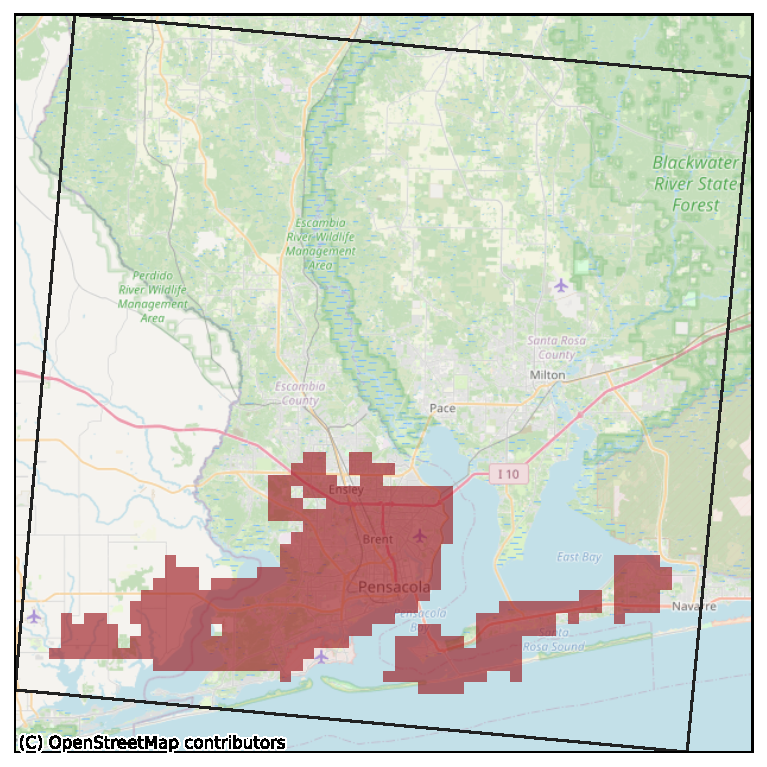
\includegraphics[width=0.22\textwidth]{figs/8_pred.pdf} \\
\end{tabular}
\caption{Pluvial NFIP claims (top) and DELUGE predictions (bottom) on seven held-out test days. Red colored cells corresponds to pixels with flood claims (top) and pixel where DELUGE predicted pluvial NFIP flood claims (bottom). DELUGE operates on $7\times 7$ patches so the three pixels at the borders are ignored.}
    \vspace{-0.15in}
\label{fig:obs-pred}
\end{figure*}
To evaluate the performance of DELUGE, we compare it against tree-based baselines, specifically Random Forest, XGBoost~\cite{chen_xgboost_2016}, and LightGBM~\cite{ke_lightgbm_2017}.
%
We focus on tree-based baselines for two reasons.
%
First, the existing ML literature on flood-damage prediction overwhelmingly relies on tabular models, with Random Forest the most commonly reported baseline~\cite{yang_predicting_2022,alipour_leveraging_2020,collins_predicting_2022,garcia_reconstructing_2025,liao_fast_2023}; we therefore include Random Forest alongside XGBoost and LightGBM as stronger tuned variants of the same family.
%
Second, while graph neural network (GNN) approaches have been proposed for flood prediction~\cite{sarkar_hydrogat_2025,kazadi_floodgnn-gru_2024,taghizadeh_interpretable_2024}, they have been developed primarily for fluvial dynamics, predicting inundation depth, and demonstrated on small catchment-scale domains, making them impractical for a CONUS-wide pluvial setting.
\paragraph{Evaluation Metrics.}Given the severe class imbalance of our problem, we use the Precision-Recall AUC (PR-AUC) as our evaluation metric.
%
In addition, we develop a dollar-weighted version of PR-AUC to account for varied range in reported flood damages.
%
To this end, we associate each positive sample with the damage density where the claim damage is equally distributed across the pixels in the claim's polygon footprint.
%
Then, integrating under a precision-recall curve where the recall is defined as the percentage of total claim dollars correctly predicted as flood claims, with precision as its standard definition, we obtain a \textbf{dollar-weighted PR-AUC metric that captures the model's ability to identify the claims weighted by claimed damages.}
%
Under this metric, we evaluate the performance of our model in terms of its ability to capture the most costly flood claims, which is of interest to insurance companies and other stakeholders.

\vspace{-5pt}
\subsection{Comparison against Baselines}Table~\ref{tab:comparison} presents the headline performance comparison between DELUGE and baseline models.
%
% tree based models dont really take in time series
Since tree-based models do not natively handle time-series or spatial rasters, we use the same set of features as introduced in \S\ref{ssec:arch-inputs}, but with some modifications to make them compatible with tree-based models.
%
For the hydrometeorological time-series, we extract the daily sum and daily max for each of the hydrometeorological features as often done in literature~\cite{yang_predicting_2022, alipour_leveraging_2020} and the center pixel value and the spatial mean for all other features in the given patch. 
%
We tuned the tree-based baselines (RF, XGBoost, LightGBM) by randomized search over 50 configurations.

\textbf{DELUGE outperforms all three baselines on both metrics}, with LightGBM the strongest tree baseline (Table~\ref{tab:comparison}).
% , LightGBM close behind, and Random Forest lagging substantially 
%
% Because each comparison shares the same splits, $\Delta\%$ is the mean per-seed difference rather than a ratio of marginal means, and DELUGE leads every baseline on this paired basis, so the overlapping absolute error bars reflect shared seed-to-seed variance rather than ambiguity in the ranking.
Because every method is evaluated on the same splits, $\Delta\%$ is a mean per-seed difference rather than a ratio of marginal means.
%
DELUGE leads every baseline on this paired basis, so the overlapping absolute-error bars reflect shared seed-to-seed variance, not ambiguity in the ranking.
%
The relative gap widens on the dollar-weighted metric, with the tree baselines trailing DELUGE by \tsim$9$ to $30\%$ on \$-Weighted PR-AUC versus \tsim$6$ to $27\%$ on PR-AUC.
%
This pattern suggests that \textbf{DELUGE's architecture helps capture the high-cost claims that tabular baselines under-predict}, the regime most relevant to insurance and emergency-management stakeholders.
%
Figure~\ref{fig:obs-pred} shows observed claims alongside DELUGE predictions drawn from the held-out spatial split.

\begin{table}[]
\small
\centering
\setlength{\tabcolsep}{4pt}
\begin{tabular}{l r r r r}
\toprule
\textbf{Model} & \textbf{PR-AUC} & \textbf{$\Delta\%$} & \textbf{\$-W PR-AUC} & \textbf{$\Delta\%$} \\
\midrule
\textbf{DELUGE (Ours)} & $\mathbf{0.243_{\pm 0.007}}$ & --      & $\mathbf{0.594_{\pm 0.049}}$ & --      \\
Random Forest          & $0.177_{\pm 0.014}$          & $-27\%$ & $0.413_{\pm 0.016}$          & $-30\%$ \\
XGBoost~\cite{chen_xgboost_2016}                & $0.219_{\pm 0.006}$          & $-10\%$  & $0.511_{\pm 0.018}$          & $-14\%$ \\
LightGBM~\cite{ke_lightgbm_2017}               & $0.228_{\pm 0.015}$          & $-6\%$ & $0.538_{\pm 0.030}$          & $-9\%$ \\
\bottomrule
\end{tabular}
\caption{\textbf{Comparison of DELUGE against tree-based baselines.} PR-AUC measures binary damage-occurrence prediction, and \$-Weighted PR-AUC weights predictions by claim amount. At a \tsim$0.25\%$ prevalence, DELUGE shows a \tsim$100$x improvement over chance performance. Scores are reported over three matched spatial splits, and $\Delta\%$ is each baseline's mean per-seed relative change from DELUGE. }
\label{tab:comparison}
\end{table}
\paragraph{Operating-Point Analysis.}
To probe how this dollar concentration manifests at fixed alert budgets, we report top-$K$ recall at several values of $K$ (Table~\ref{tab:topk}), separating occurrence recall (R@K) from dollar recall (\$R@K).
%
At every $K$, \$R@K sharply exceeds R@K.
%
At $K=0.1\%$ DELUGE captures only $19\%$ of pluvial claim events but $62\%$ of total damage dollars and at $K=1\%$ the gap remains ($52\%$ events vs.\ $90\%$ dollars).
%
DELUGE also leads both XGBoost and LightGBM at every $K$ on both metrics, with the largest gap at the tightest, most operationally relevant budgets.
%
\textbf{DELUGE's top-ranked predictions are therefore concentrated in the high-cost regime}, the operationally meaningful slice of the test set for insurance and emergency-management workflows.

\vspace{5pt}
\begin{table}[h]
\small
\centering
\setlength{\tabcolsep}{4pt}
\begin{tabular}{l rr rr rr}
\toprule
& \multicolumn{2}{c}{\textbf{DELUGE}} & \multicolumn{2}{c}{XGBoost} & \multicolumn{2}{c}{LightGBM} \\
\cmidrule(lr){2-3}\cmidrule(lr){4-5}\cmidrule(lr){6-7}
$\boldsymbol{K}$ & R@K & \$R@K & R@K & \$R@K & R@K & \$R@K \\
\midrule
$0.1\%$ & $\mathbf{0.193}$ & $\mathbf{0.617}$ & 0.173 & 0.609 & 0.180 & 0.557 \\
$0.2\%$ & $\mathbf{0.279}$ & $\mathbf{0.728}$ & 0.257 & 0.701 & 0.260 & 0.668 \\
$0.5\%$ & $\mathbf{0.412}$ & $\mathbf{0.832}$ & 0.388 & 0.813 & 0.391 & 0.803 \\
$1\%$   & $\mathbf{0.521}$ & $\mathbf{0.897}$ & 0.495 & 0.880 & 0.500 & 0.872 \\
\bottomrule
\end{tabular}
\caption{Top-$K$ recall. R@K is occurrence recall at $K$ (fraction of positive pixel-days captured) and \$R@K is dollar recall at $K$ (fraction of total claim dollars captured). $K$ given as a percentile of the held-out pixel-day test set.}
% \fix{adding error bars}}
\label{tab:topk}
\end{table}
\vspace{-5pt}
\subsection{Ablation Studies}
We ablate DELUGE along two axes (Table~\ref{tab:ablations}). \emph{Module ablations} swap out our architectural contributions and \emph{feature ablations} drop one input modality at a time while leaving the architecture intact.
%
\paragraph{Modulator Ablations.} We replace our modulator-based encoder with a standard ConvLSTM and a Transformer, common architectures for spatiotemporal data, applied to the hydrometeorological time-series.
%
DELUGE performs on par with both alternatives on mean, with the Transformer marginally ahead on PR-AUC and DELUGE marginally ahead on \$-Weighted PR-AUC, while ConvLSTM trails slightly on both.
%
\textbf{Our modulator design therefore retains predictive accuracy comparable to stronger sequence-model alternatives while adding \emph{interpretability-by-design}.}
%
We then progressively ablate the modulators' conditioning, from frozen at initialization (Uniform), to learnable but globally shared, to per-patch conditioned on a single channel (AEF-only or Terrain-only).
%
Each step closes part of the gap to full DELUGE on both metrics, confirming that \textbf{both learning the modulator parameters and conditioning them per patch matter}.
%
AEF-only and Terrain-only perform nearly identically on PR-AUC, with AEF-only modestly stronger on \$-Weighted PR-AUC, suggesting the two conditioning channels carry largely overlapping information about local hydrology.
%
\textbf{This demonstrates the utility of AlphaEarth embeddings for pluvial flood prediction.} As a conditioning signal they perform on par with a curated suite of hydrological terrain descriptors and well above unconditioned modulators, with no hydrological feature engineering required.

\vspace{-3pt}
\paragraph{Feature Ablations.} The single largest drop comes from removing the hydrometeorological hazard inputs (precipitation, soil moisture, and snow water equivalent), which collapses the model and \textbf{confirms hydrometeorology as the dominant driver of DELUGE's prediction}.
%
Among the remaining modalities, Exposure shows the largest gap, reflecting its role in identifying which structures sit in the path of damaging precipitation.
%
% Interestingly, removing terrain features together with the AlphaEarth embedding (the modulators' conditioning input) costs a comparable $-$10\% / $-$11\%, but notably smaller than the Uniform Modulators gap above, suggesting that terrain and AlphaEarth contribute more strongly through the modulators than as direct fused features.
%
Vulnerability shows the smallest gap, suggesting structural attributes carry less independent signal, perhaps as they correlate with AlphaEarth~\cite{bell_earth_2026}.



\begin{table}[ht]
\centering
\small
\setlength{\tabcolsep}{3pt}
\begin{tabular}{l r r r r}
\toprule
\textbf{Configuration} & \textbf{PR-AUC} & \textbf{$\Delta\%$} & \textbf{\$-W PR-AUC} & \textbf{$\Delta\%$} \\
\midrule
\textbf{DELUGE (Full)} & $\mathbf{0.243_{\pm 0.007}}$ & -- & $\mathbf{0.594_{\pm 0.049}}$ & -- \\
\midrule
\multicolumn{5}{l}{\emph{Module ablations}} \\
\, Uniform Modulators     & $0.196_{\pm 0.014}$ & $-$19\% & $0.414_{\pm 0.050}$ & $-$30\%  \\
\, Globally-shared Modulators & $0.217_{\pm 0.011}$ & $-$11\% & $0.528_{\pm 0.053}$ & $-$11\% \\
\, AEF-only Modulators & $0.234_{\pm 0.016}$ & $-$4\% & $0.572_{\pm 0.081}$ & $-$4\% \\
\, Terrain-only Modulators & $0.235_{\pm 0.012}$ & $-$3\% & $0.558_{\pm 0.073}$ & $-$6\% \\
\addlinespace[0.3em]
\hdashline[2pt/2pt]
\addlinespace[0.3em]
\, ConvLSTM Hydromet.   & $0.234_{\pm 0.014}$ & $-$4\% & $0.543_{\pm 0.089}$ & $-$9\% \\
\, Transformer Hydromet.   & $0.250_{\pm 0.029}$ & $+$3\% & $0.574_{\pm 0.119}$ & $-$4\% \\
\midrule
\multicolumn{5}{l}{\emph{Feature ablations}} \\
\, Exposure       & $0.217_{\pm 0.017}$ & $-$11\% & $0.476_{\pm 0.071}$ & $-$20\% \\
\, Vulnerability  & $0.229_{\pm 0.012}$ & $-$6\% & $0.526_{\pm 0.056}$ & $-$11\% \\
\, Terrain Hazard & $0.218_{\pm 0.007}$ & $-$11\% & $0.496_{\pm 0.078}$ & $-$17\% \\
\, Hydromet. Hazard & $0.020_{\pm 0.002}$ & $-$92\% & $0.038_{\pm 0.008}$ & $-$94\% \\
\bottomrule
\end{tabular}
\caption{\textbf{Module and feature ablations of DELUGE.} Each row removes or replaces the listed component from the full model. 
%
Module ablations swap an architectural component while feature ablations drop one input modality while leaving the architecture intact. 
% The Terrain Hazard ablation removes terrain features together with the AlphaEarth embedding, since they jointly condition the modulators. 
}
\label{tab:ablations}
\end{table}

\begin{figure*}[!ht]
\centering
\setlength{\tabcolsep}{1pt}
\renewcommand{\arraystretch}{0.4}
\begin{tabular}{ccccc}
% \rotatebox{90}{\,\textbf{Basemap}} &
% 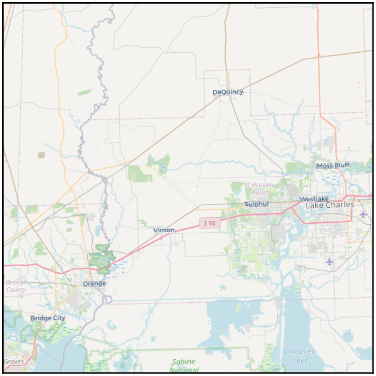
\includegraphics[width=0.18\textwidth]{figs/cell_dynamics_val_cell_1331_basemap.pdf} &
% 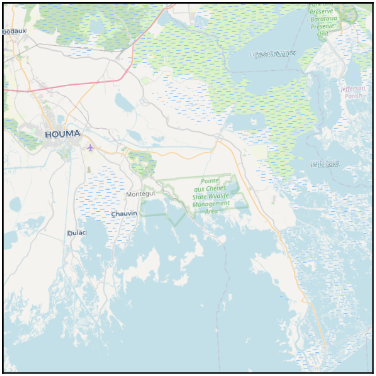
\includegraphics[width=0.18\textwidth]{figs/cell_dynamics_val_cell_1486_basemap.pdf} &
% 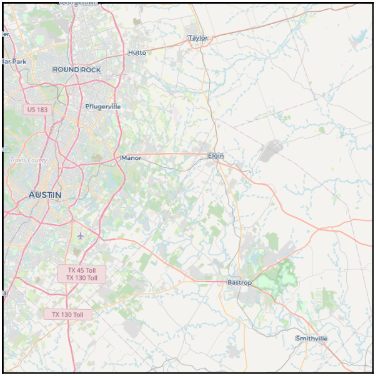
\includegraphics[width=0.18\textwidth]{figs/cell_dynamics_val_cell_1136_basemap.pdf} &
% 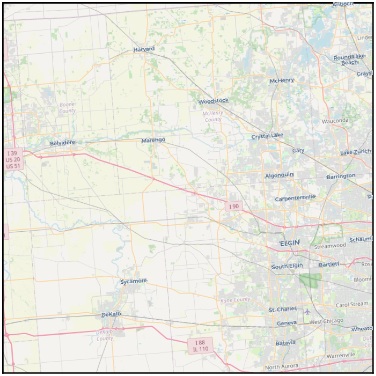
\includegraphics[width=0.18\textwidth]{figs/cell_dynamics_val_cell_1544_basemap.pdf} &
% 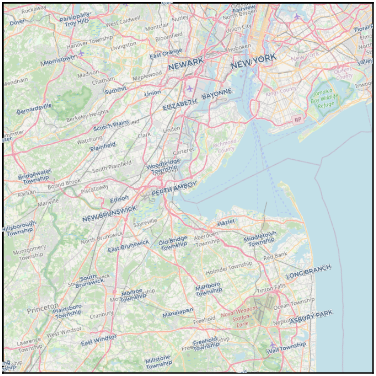
\includegraphics[width=0.18\textwidth]{figs/cell_dynamics_val_cell_2168_basemap.pdf} \\
% \rotatebox{90}{\,\textbf{Dynamics}} &
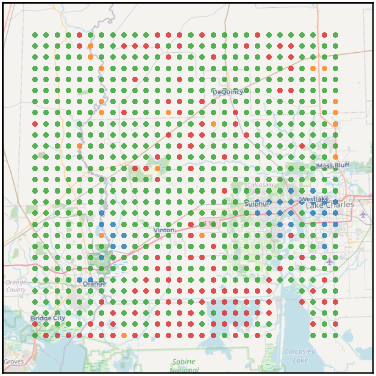
\includegraphics[width=0.19\textwidth]{figs/cell_dynamics_val_cell_1331.pdf} &
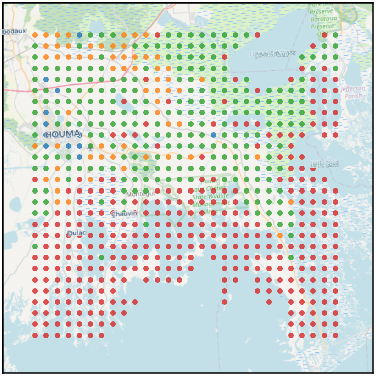
\includegraphics[width=0.19\textwidth]{figs/cell_dynamics_val_cell_1486.pdf} &
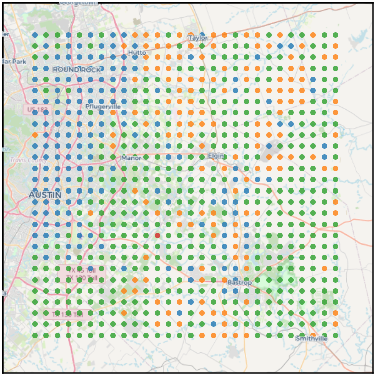
\includegraphics[width=0.19\textwidth]{figs/cell_dynamics_val_cell_1136.pdf} &
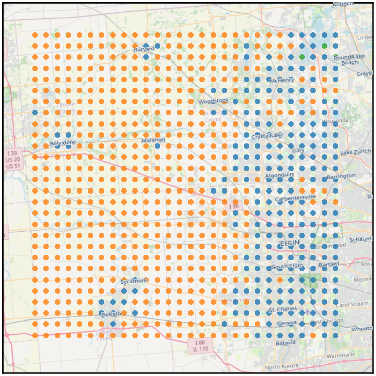
\includegraphics[width=0.19\textwidth]{figs/cell_dynamics_val_cell_1544.pdf} &
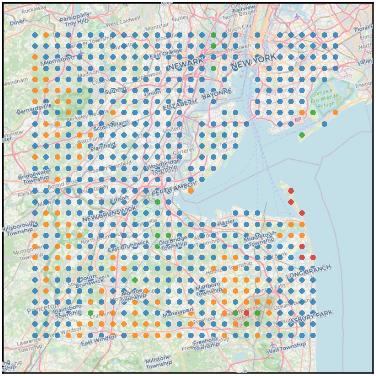
\includegraphics[width=0.19\textwidth]{figs/cell_dynamics_val_cell_2168.pdf} \\
 % & (a) & (b) & (c) & (d) & (e) \\
\end{tabular}
% \caption{Basemap (top) and learned modulator dynamics clustering result (bottom) for five representative held-out cells (\S\ref{ssec:modulator_behaviors}). Colors follows the same scheme as Fig.~\ref{fig:modulator-clusters} for consistency. Note that we take every other pixel for simplicity and clarity.}
\caption{Learned modulator dynamics clustering result for five representative held-out cells (\S\ref{ssec:modulator_behaviors}). Colors follows the same scheme as Fig.~\ref{fig:modulator-clusters} for consistency.}
    \vspace{-0.15in}
\label{fig:cell-dynamics}
\end{figure*}
\vspace{-3pt}
\subsection{Verifying Learned Behavior of the Modulators}\label{ssec:modulator_behaviors}
Explainability and physical fidelity are growing concerns in Geospatial AI~\cite{hsu_explainable_2023,roussel2025introducing,suri_trusting_nodate} and flood modeling~\cite{taghizadeh_interpretable_2024}.
%
While a substantial body of work examines what geospatial embeddings encode about physical space~\cite{benavides2026earth,rahman_physically_2026}, comparatively little addresses how downstream models should consume these representations in a physically verifiable manner.
%
DELUGE's modulators are designed to this end. Because their parameters constitute the model's predictive computation directly, the interpretability they afford is architectural rather than post-hoc, obtained by inspecting the learned parameters themselves rather than by explaining individual predictions.

The modulators act on the hydrometeorology branch, which our ablations also identify as the dominant predictive driver (Table~\ref{tab:ablations}), so its learned response is the most consequential to interpret.
%
For each patch, we summarize the Value Modulator's warp $\phi_{v,i}(\tilde{x})$ and Temporal Modulator's response kernel $k_v(\tau)$ by their CDFs.
%
Here, we omit snow water equivalent and focus on precipitation and soil moisture, the channels most directly relevant to pluvial flooding.
% We compute these for the two channels relevant to pluvial flooding --- precipitation and soil moisture --- omitting snow water equivalent, yielding four CDF blocks per pixel that we standardize and concatenate.
%
To cluster, we apply PCA on the CDFs down to two components (\tsim$75\%$ of variance) followed by K-means. 
%
A silhouette sweep determined $K=4$.
%
To illustrate the learned modulator behavior within each cluster, Figure~\ref{fig:cell-dynamics} shows representative held-out grid cells with their modulator dynamics clustering assignments, and Figure~\ref{fig:modulator-clusters} shows the corresponding modulator dynamics for each cluster.

First, examining the Temporal Modulator's kernel (Fig.~\ref{fig:modulator-clusters}) for 1hr acc. precip. (top) and soil moisture (bottom), we find that \textbf{DELUGE learns to rely on precipitation for the immediate risk and soil moisture to capture antecedent conditions}, with the latter kernels peaking in the \tsim$7-15$ hour range in contrast with the precipitation kernels that peak at $\tau\approx0$ and decay rapidly.
%
Notice in Fig~\ref{fig:modulator-clusters} that within \emph{every} cluster the two kernels are cleanly staggered, with the precipitation kernel concentrated at the most recent hour and the soil-moisture kernel peaking several hours later, an explicit hand-off from instantaneous precipitation forcing to antecedent wetness state that DELUGE recovers without a hydrological prior.
%
Next, with a further qualitative inspection of the clustering results, we derive the characters of the four identified clusters.

\begin{figure}[]
\centering
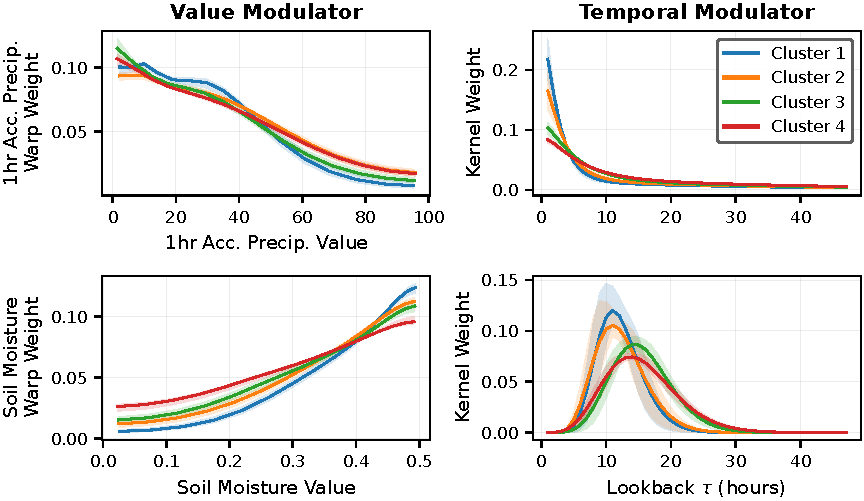
\includegraphics[width=\columnwidth]{figs/modulator_clusters.pdf}
\caption{Clusters identified in modulator-parameter space ($K=4$) and their corresponding modulator dynamics.}
% \vspace{-10pt}
\label{fig:modulator-clusters}
\end{figure}
%
% \begin{enumerate}[nosep, align=left, leftmargin=*, left=0pt]

\noindent
\colorchip{1f77b4}\,\,\textbf{Cluster 1} (Blue) corresponds to denser urban areas, with a sharp reliance on recent precipitation. This short lag time aligns with how impervious surfaces accelerate runoff yield~\cite{liao_fast_2023}. Furthermore, it shows higher importance of lower precipitation than others, signaling its relative vulnerability to lower precipitation and relies on relatively recent soil moisture with emphasis on the higher soil moisture values.

\noindent
\colorchip{ff7f0e}\,\,\textbf{Cluster 2} (Orange) corresponds to suburban areas in inland regions of CONUS, with moderate reliance on recent precipitation. Soil moisture kernel is similar to cluster 1, with a slightly even emphasis on all soil moisture values.

\noindent
\colorchip{2ca02c}\,\,\textbf{Cluster 3} (Green) corresponds to suburban areas along the Gulf, with a longer tail of precipitation kernel and a longer and wider lookback range than the first two clusters. Its characteristics lie in the middle of the clusters 2 and 4 drawing on both the suburban and water-facing characteristics.

\noindent
\colorchip{d62728}\,\,\textbf{Cluster 4} (Red) corresponds to water-facing regions. Represented by the longest tail in the precipitation kernel and the widest lookback range in the soil moisture kernel, this cluster also places the most even importance in soil moisture values. This may suggest water-facing regions are more susceptible to flooding even when the top layer of soil is not saturated due to the high water table.

We emphasize that the value of this result lies not in the clusters aligning with geography.
%
Such alignment is unsurprising, since the modulators are conditioned on foundation-model embeddings and terrain descriptors that already encode geographic structure.
%
It lies instead in the fact that the \textbf{clusters admit a coherent hydrological interpretation}, the architecture-level interpretability we set out to establish, which allows the physical fidelity of the foundation-model conditioning to be assessed directly from the learned parameters.
%
More broadly, \textbf{we view this conditioning scheme as not unique to pluvial flooding but applicable to other geospatial tasks that build on Geospatial Foundation Models}, where routing embeddings through physically meaningful parametric modules can make the model's use of them directly inspectable.
%
The full clustering results are placed in the Appendix.
%

\vspace{-6pt}
\subsection{Failure Modes}
\label{ssec:failure-modes}
% We observe two recurring main failure modes.
     \paragraph{Low-damage claims are harder to predict.} These claims are often associated with less anomalous hydrometeorological conditions, making them more difficult to distinguish from non-damage cases. 
        %
        To characterize this quantitatively, we stratify held-out claim-days by claim amount (Table~\ref{tab:damage-severity}). 
        %
        PR-AUC rises sharply from the smallest bin to the [\$50K, \$500K) tier ($0.04\to0.37$), with \$-Weighted PR-AUC tracking the same trend. The slight drop in the largest [\$500K, $\infty$) tier reflects its extreme base rate (0.004\%) rather than degraded ranking. 
        %
        \textbf{DELUGE is therefore strongest in the high-cost regime most relevant to insurance and emergency management stakeholders}.
        % while underperforming in the low-cost regime.
\begin{table}[h]
\centering
\small
\setlength{\tabcolsep}{4pt}
\begin{tabular}{l r r r}
\toprule
\textbf{Damage range (\$)} & \textbf{Prev. (\%)} & \textbf{PR-AUC} & \textbf{\$-W PR-AUC} \\
\midrule
{}[0, 5{,}000)              & 0.124  & 0.043 & 0.049 \\
{}[5{,}000, 50{,}000)       & 0.087  & 0.154 & 0.186 \\
{}[50{,}000, 500{,}000)     & 0.030  & 0.368 & 0.424 \\
{}[500{,}000, $\infty$)     & 0.004  & 0.313 & 0.331 \\
\bottomrule
\end{tabular}
\caption{\textbf{DELUGE performance stratified by claim amount.} Per-bin prevalence, PR-AUC, and dollar-weighted PR-AUC on a single held-out spatial split.}
\label{tab:damage-severity}
\end{table}

\begin{figure}[]
\centering
\setlength{\tabcolsep}{1pt}
\renewcommand{\arraystretch}{0.2}
\begin{tabular}{c@{\hspace{1pt}}cccc}
\rotatebox{90}{\,\textbf{NFIP Claims}} &
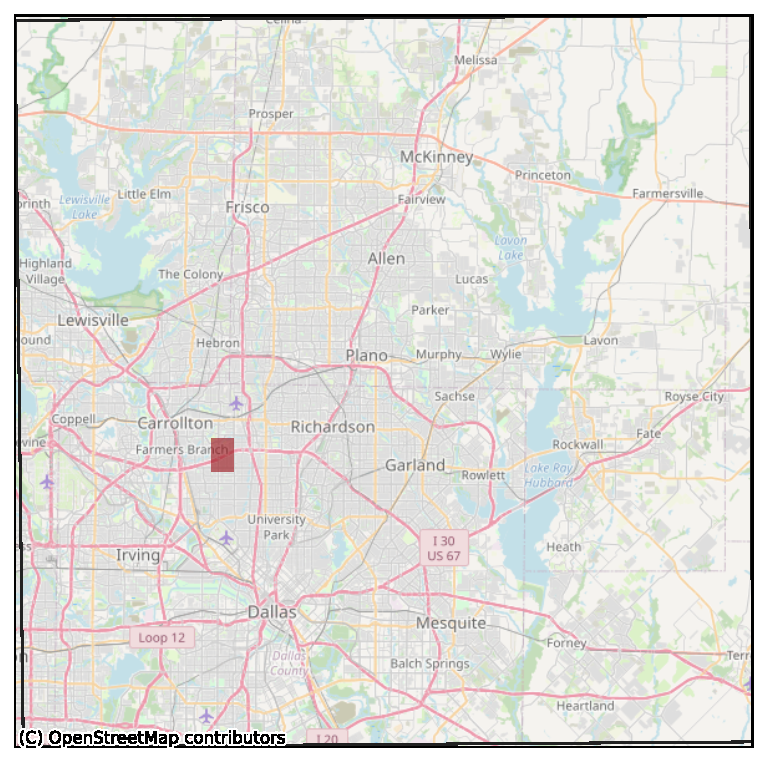
\includegraphics[width=0.24\columnwidth]{figs/fail_1_obs.pdf} &
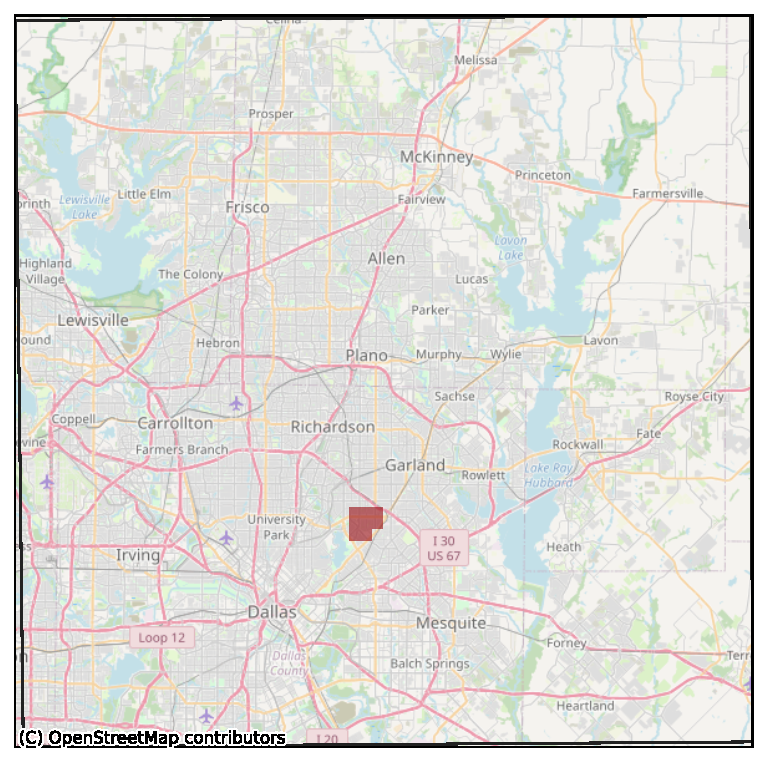
\includegraphics[width=0.24\columnwidth]{figs/fail_2_obs.pdf} &
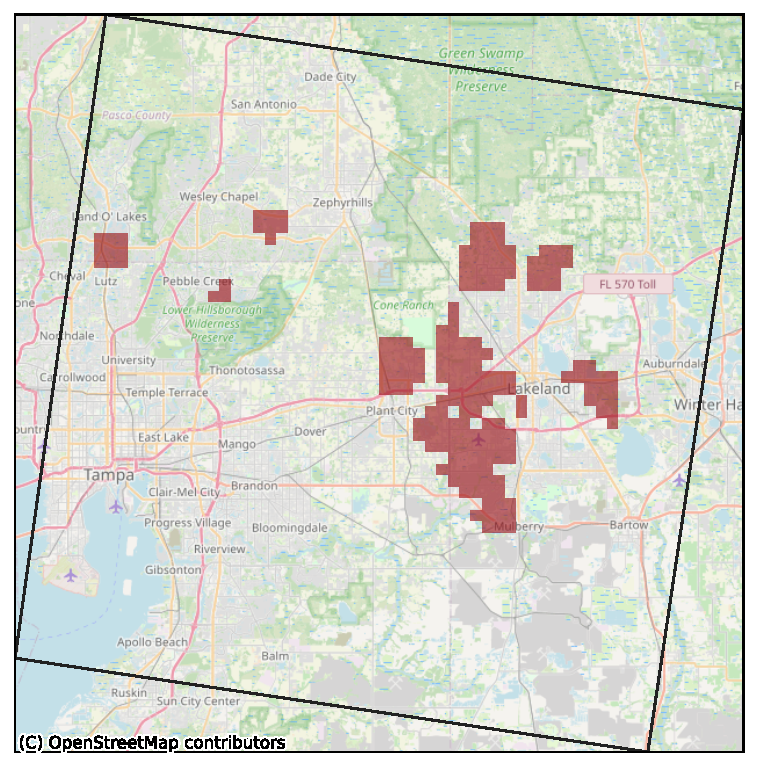
\includegraphics[width=0.24\columnwidth]{figs/fail_3_obs.pdf} &
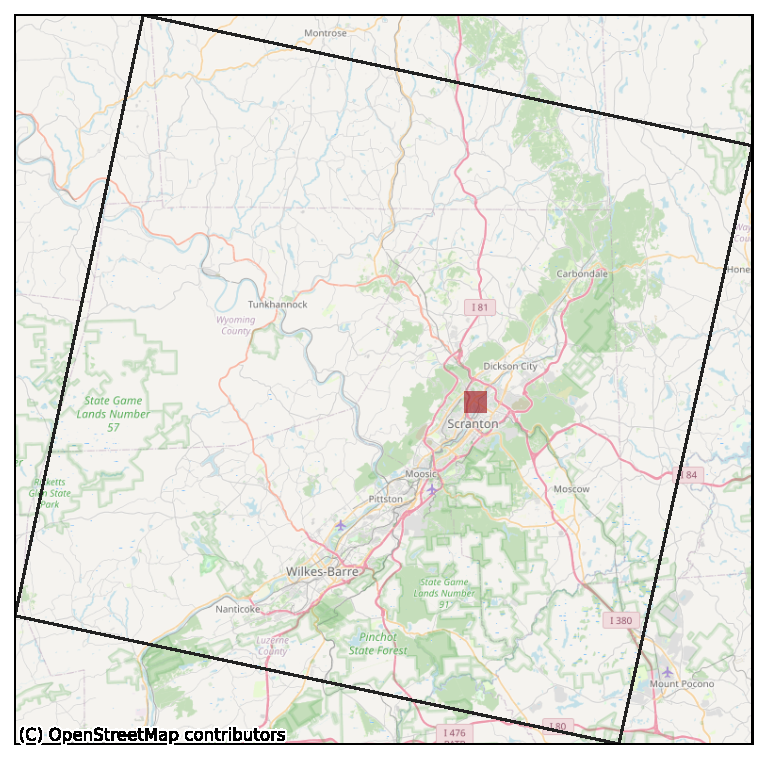
\includegraphics[width=0.24\columnwidth]{figs/fail_4_obs.pdf} \\
\rotatebox{90}{\,\textbf{Predicted}} &
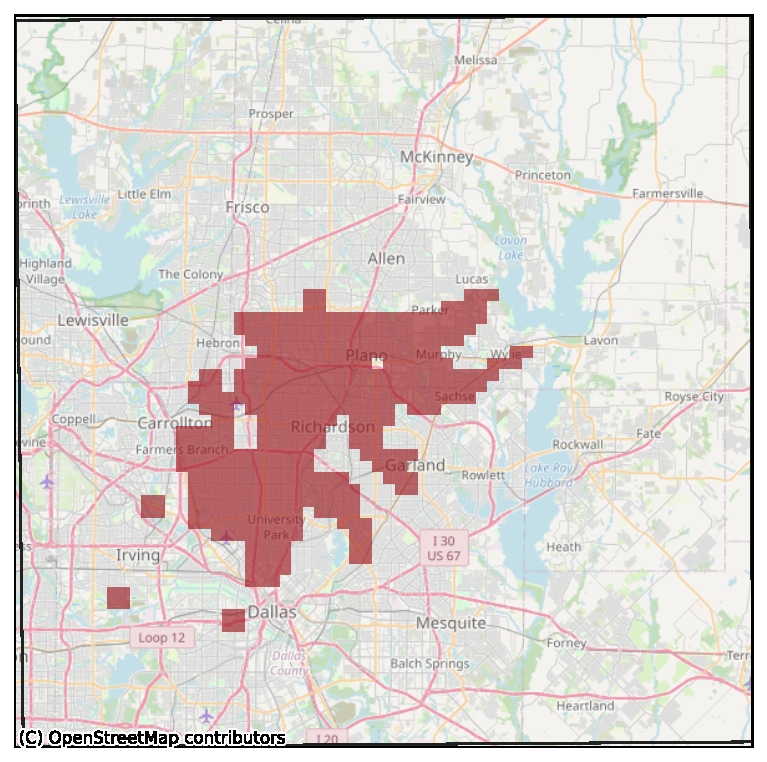
\includegraphics[width=0.24\columnwidth]{figs/fail_1_pred.pdf} &
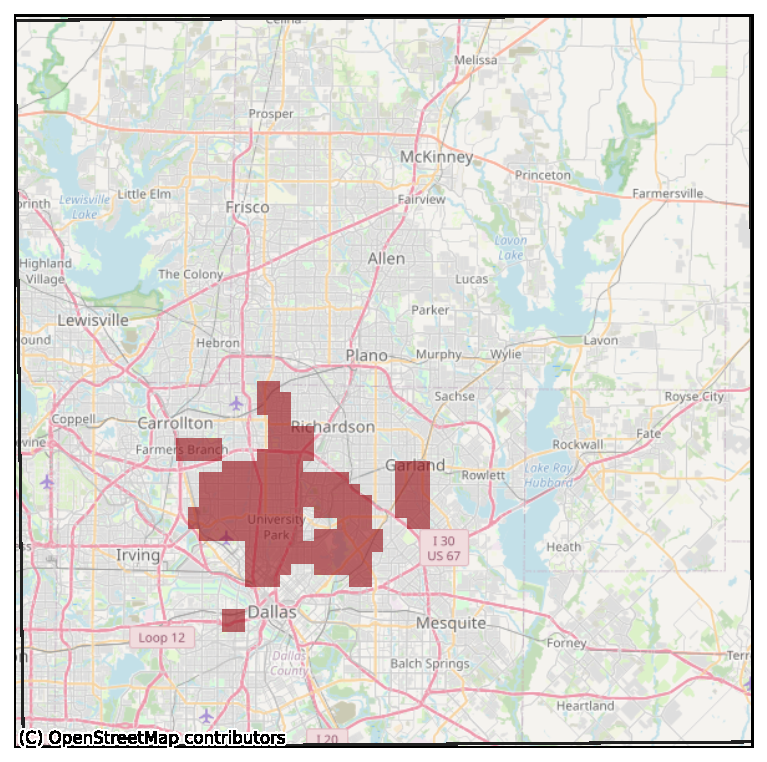
\includegraphics[width=0.24\columnwidth]{figs/fail_2_pred.pdf} &
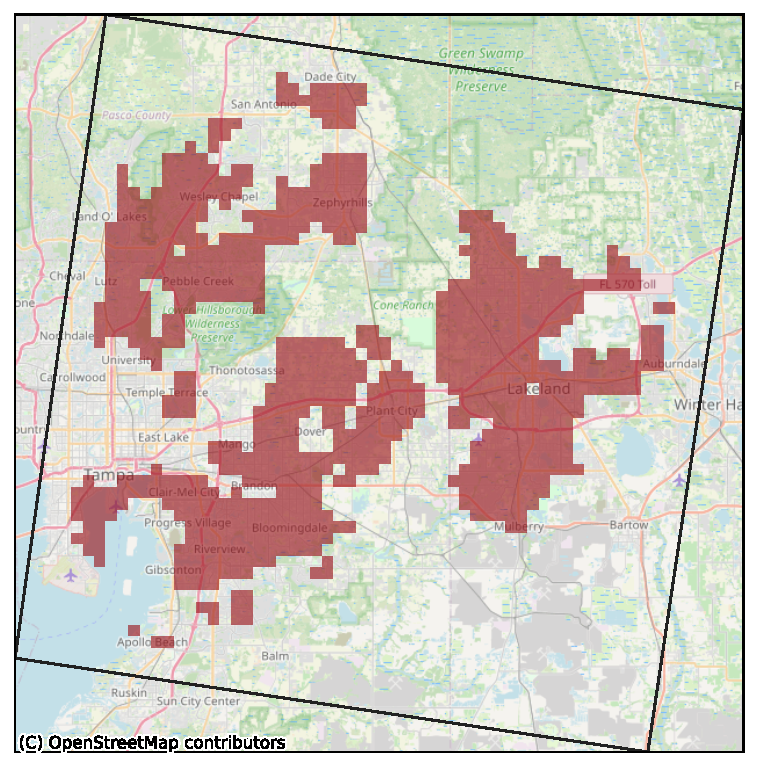
\includegraphics[width=0.24\columnwidth]{figs/fail_3_pred.pdf} &
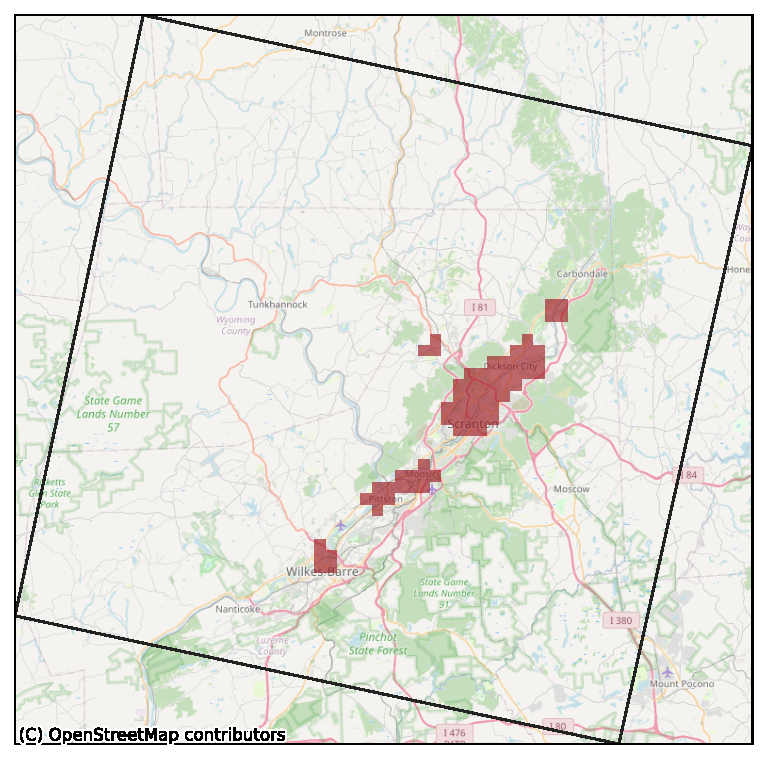
\includegraphics[width=0.24\columnwidth]{figs/fail_4_pred.pdf} \\
                                                               % & (a) & (b) & (c) & (d)\\
\end{tabular}
\caption{DELUGE dense urban failure cases NFIP claims and DELUGE predictions  on four held-out test days where DELUGE fails to pinpoint flood claims in urban areas.}
\label{fig:failure-modes}
\end{figure}
% \vspace{-5pt}
\paragraph{Locations of impacts of large storm systems with widespread precipitation are hard to resolve.}
% \paragraph{Large storm systems with widespread precipitation are hard to localize in their impact.}
%
Pinpointing which pixels experience damage is difficult, especially in dense urban areas where flood response is governed by fine-scale local processes.
%
Figure~\ref{fig:failure-modes} shows representative cases where DELUGE registers that a large storm system causes damage but struggles to localize exactly which urban pixels are affected.
%
We attribute this to two factors.
%
First, because we predict only \emph{insured} damage reported through NFIP, some pixels in our negative class may have experienced unreported damage, blurring the supervisory signal.
%
Second, and independent of this, dense urban areas are where we most consistently observe DELUGE to struggle, as we show by stratifying performance over AEF-defined location characteristics in the Appendix.
%
We anticipate that higher spatial (sub-kilometer) and temporal (sub-hourly) resolution hydrometeorology will be needed to resolve fine-scale urban damage.
